\documentclass{standalone}
\usepackage[utf8]{inputenc}

\usepackage{tikz}
\usetikzlibrary{positioning, arrows, fit, calc}
\begin{document}

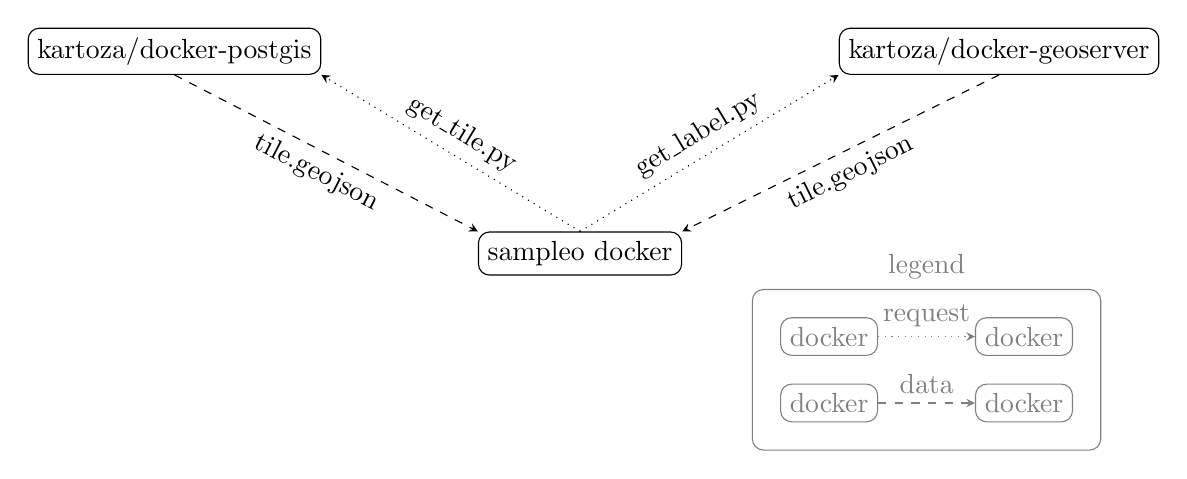
\begin{tikzpicture}[node distance=8em]
	
	\tikzstyle{node}=[draw, rounded corners]
	\tikzstyle{legendbox}=[draw, rounded corners, inner sep=10pt]
    
    \tikzstyle{request}=[-stealth, dotted]
    \tikzstyle{data}=[-stealth, dashed]


	\node[node](sampleo){sampleo docker};
    
    
    \node[node, above left=of sampleo](pg){kartoza/docker-postgis};
    \node[node, above right=of sampleo](gs){kartoza/docker-geoserver};
    
    \draw[request] (sampleo.north) -- (gs.south west) node [midway,above, sloped]{get\_label.py};
    \draw[request] (sampleo.north) -- (pg.south east) node [midway,above, sloped]{get\_tile.py};
    
    \draw[data, xshift=1em] (pg.south) -- (sampleo.north west) node [midway,below, sloped]{tile.geojson};
    
    \draw[data, xshift=1em] (gs.south) -- (sampleo.north east) node [midway,below, sloped]{tile.geojson};
    
    
    % legend
    \begin{scope}[xshift=9em, yshift=-3em, node distance=1em and 3.5em, draw=gray, text=gray]
    \node[node] (legend_serv11) {docker};
    \node[node, right=of legend_serv11] (legend_serv21) {docker};
    
    \draw[request] (legend_serv11) -- (legend_serv21) node [midway, above]{request};
    
    \node[node, below=of legend_serv11] (legend_serv21) {docker};
    \node[node, right=of legend_serv21] (legend_serv22) {docker};
    
    \draw[data] (legend_serv21) -- (legend_serv22) node [midway, above]{data};
    
    \node[legendbox, fit=(legend_serv11)(legend_serv22),label=above:legend]{};
    
    \end{scope}
    
    
\end{tikzpicture}

\end{document}
